\documentclass[14pt,a4paper]{extarticle}
\usepackage{graphicx}
\usepackage{caption} 
\usepackage{hyperref}
\usepackage[T1]{fontenc}
\usepackage[utf8x]{inputenc}
\usepackage{pdfpages}
\usepackage{libertine}
\usepackage{listings}
\usepackage{xcolor}
\usepackage{enumitem}
\usepackage{fullpage}
\usepackage{ulem}
\usepackage{cancel}

\renewcommand{\thesection}{\arabic{section}}
\renewcommand{\familydefault}{\sfdefault}


\colorlet{punct}{red!60!black}
\definecolor{delim}{RGB}{20,105,176}
\colorlet{numb}{magenta!60!black}

\hypersetup{
    colorlinks=true,
    linkcolor=blue,
    filecolor=blue,      
    urlcolor=blue,
    pdfborder={0 0 0},
    linktocpage      
}

\begin{document}
	\begin{titlepage}
		\centering
		{\scshape\LARGE Blockchains \par}
		\vspace{2.5cm}
		{\huge\bfseries CryptoZombie}
		\vfill
		{\normalsize von\par}
		{\normalsize Benjamin Ellmer (\textsc{S2210455012}) \par}
		\vspace{1cm}
		
\includegraphics[width=0.3\textheight]{images/logo.pdf} \par
		\vspace{1cm}
		{\large Mobile Computing Master \par}
		{\large FH Hagenberg \par}
		\vfill
		{\large \today\par}
	\end{titlepage}

	\section*{Source Code}
	You can find the code for all lessons in the submission folder.

	\section*{Lesson 1}
	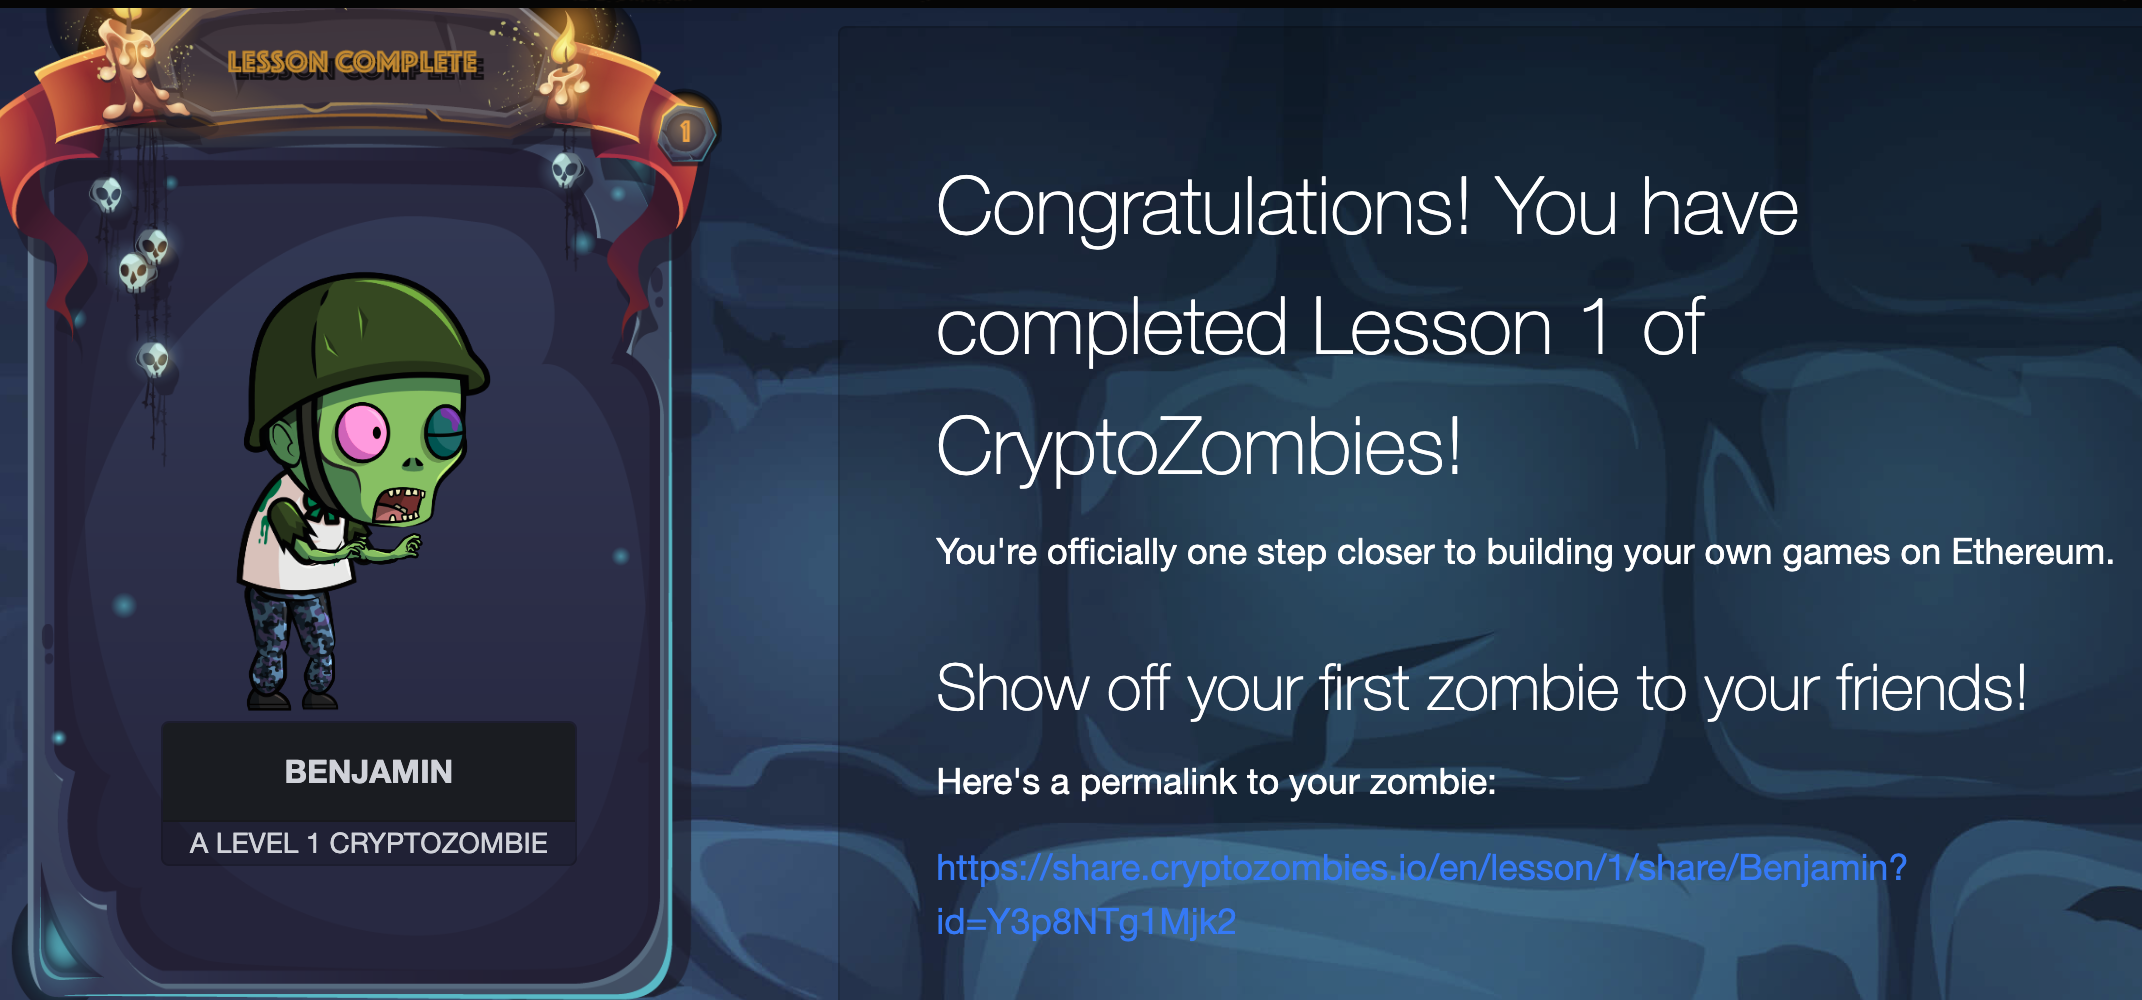
\includegraphics[width=\textwidth]{images/lesson1.png}

	\section*{Lesson 2}
	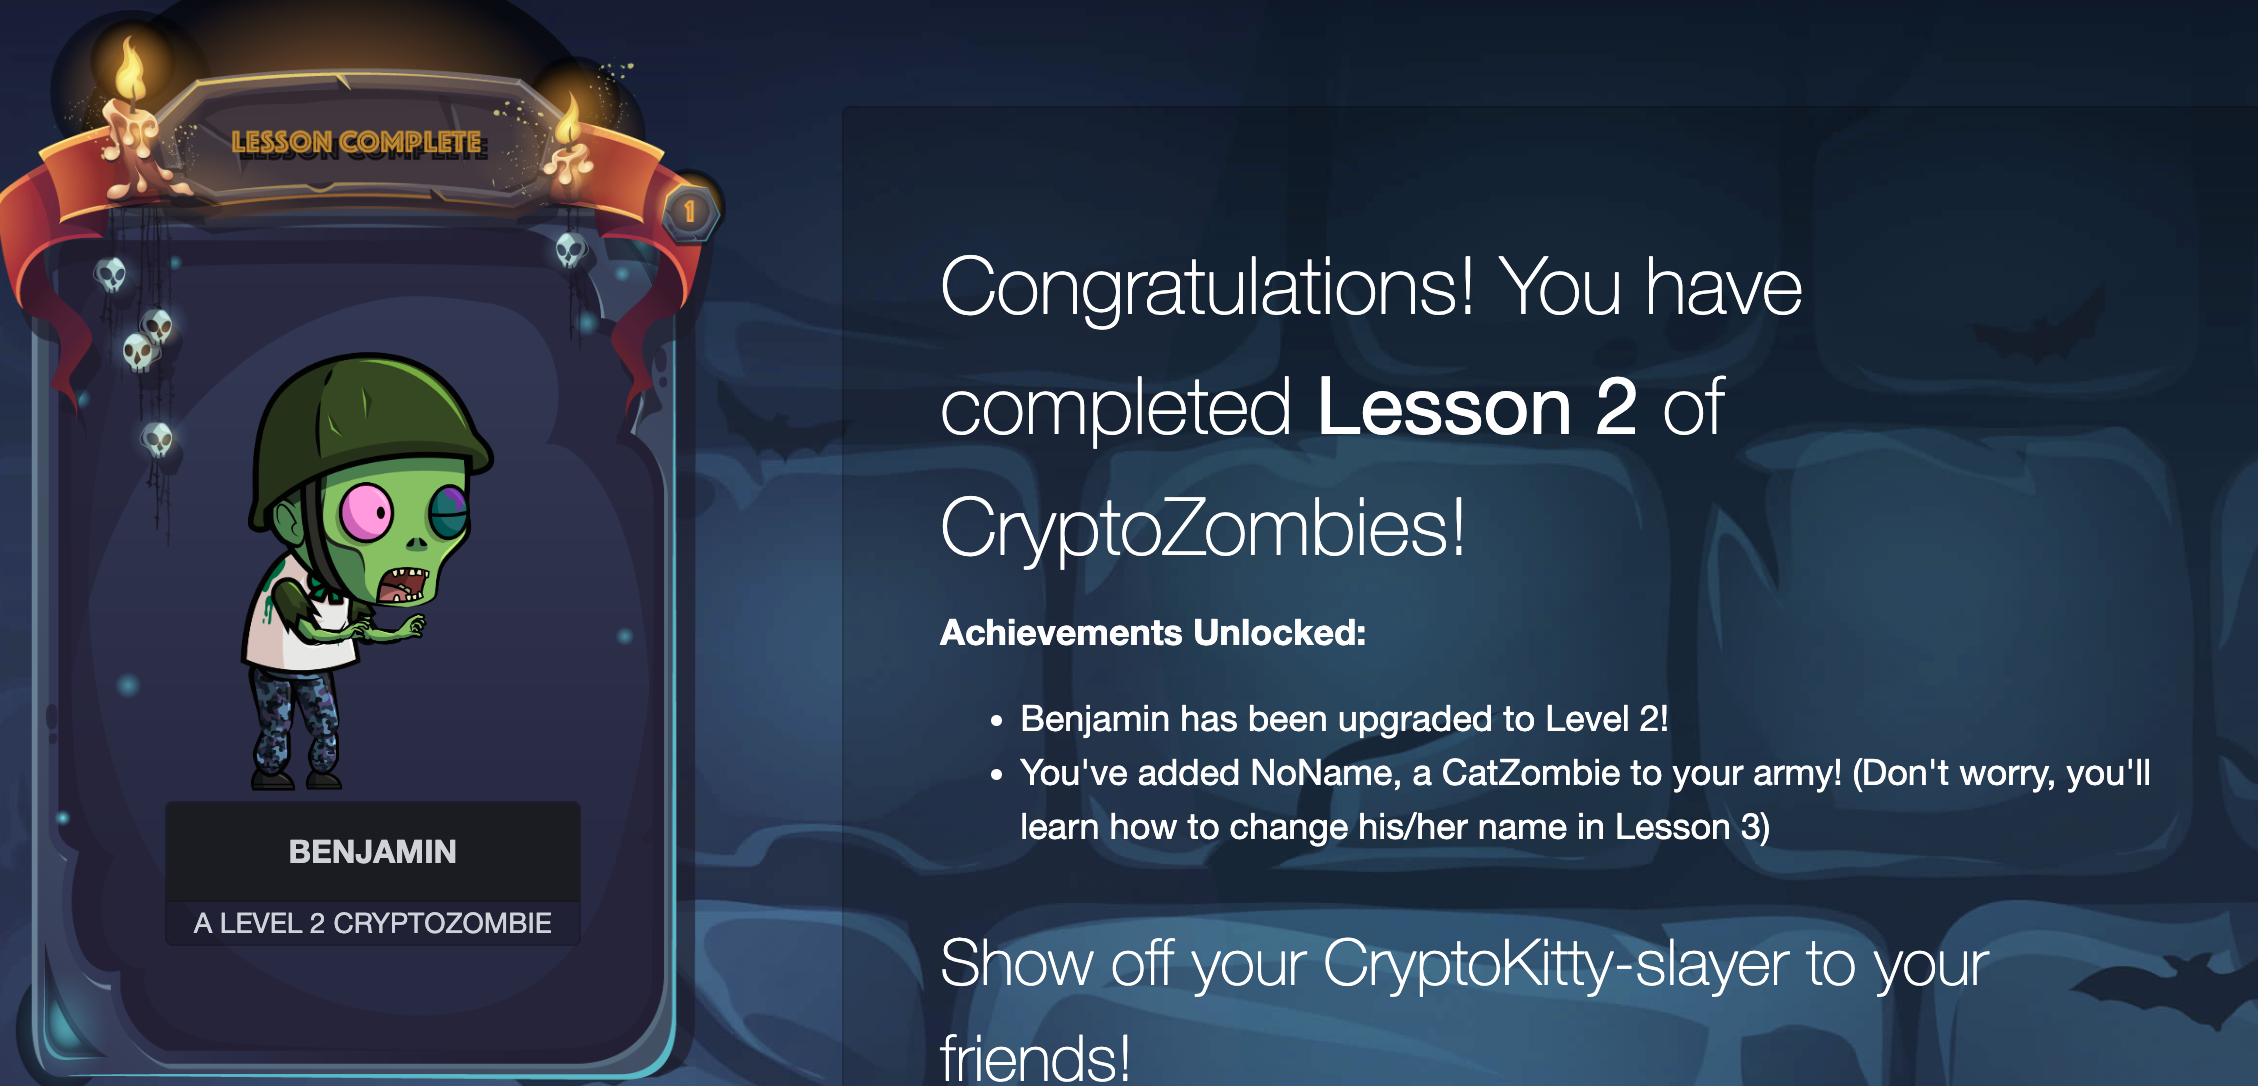
\includegraphics[width=\textwidth]{images/lesson2.png}

	\section*{Lesson 3}
	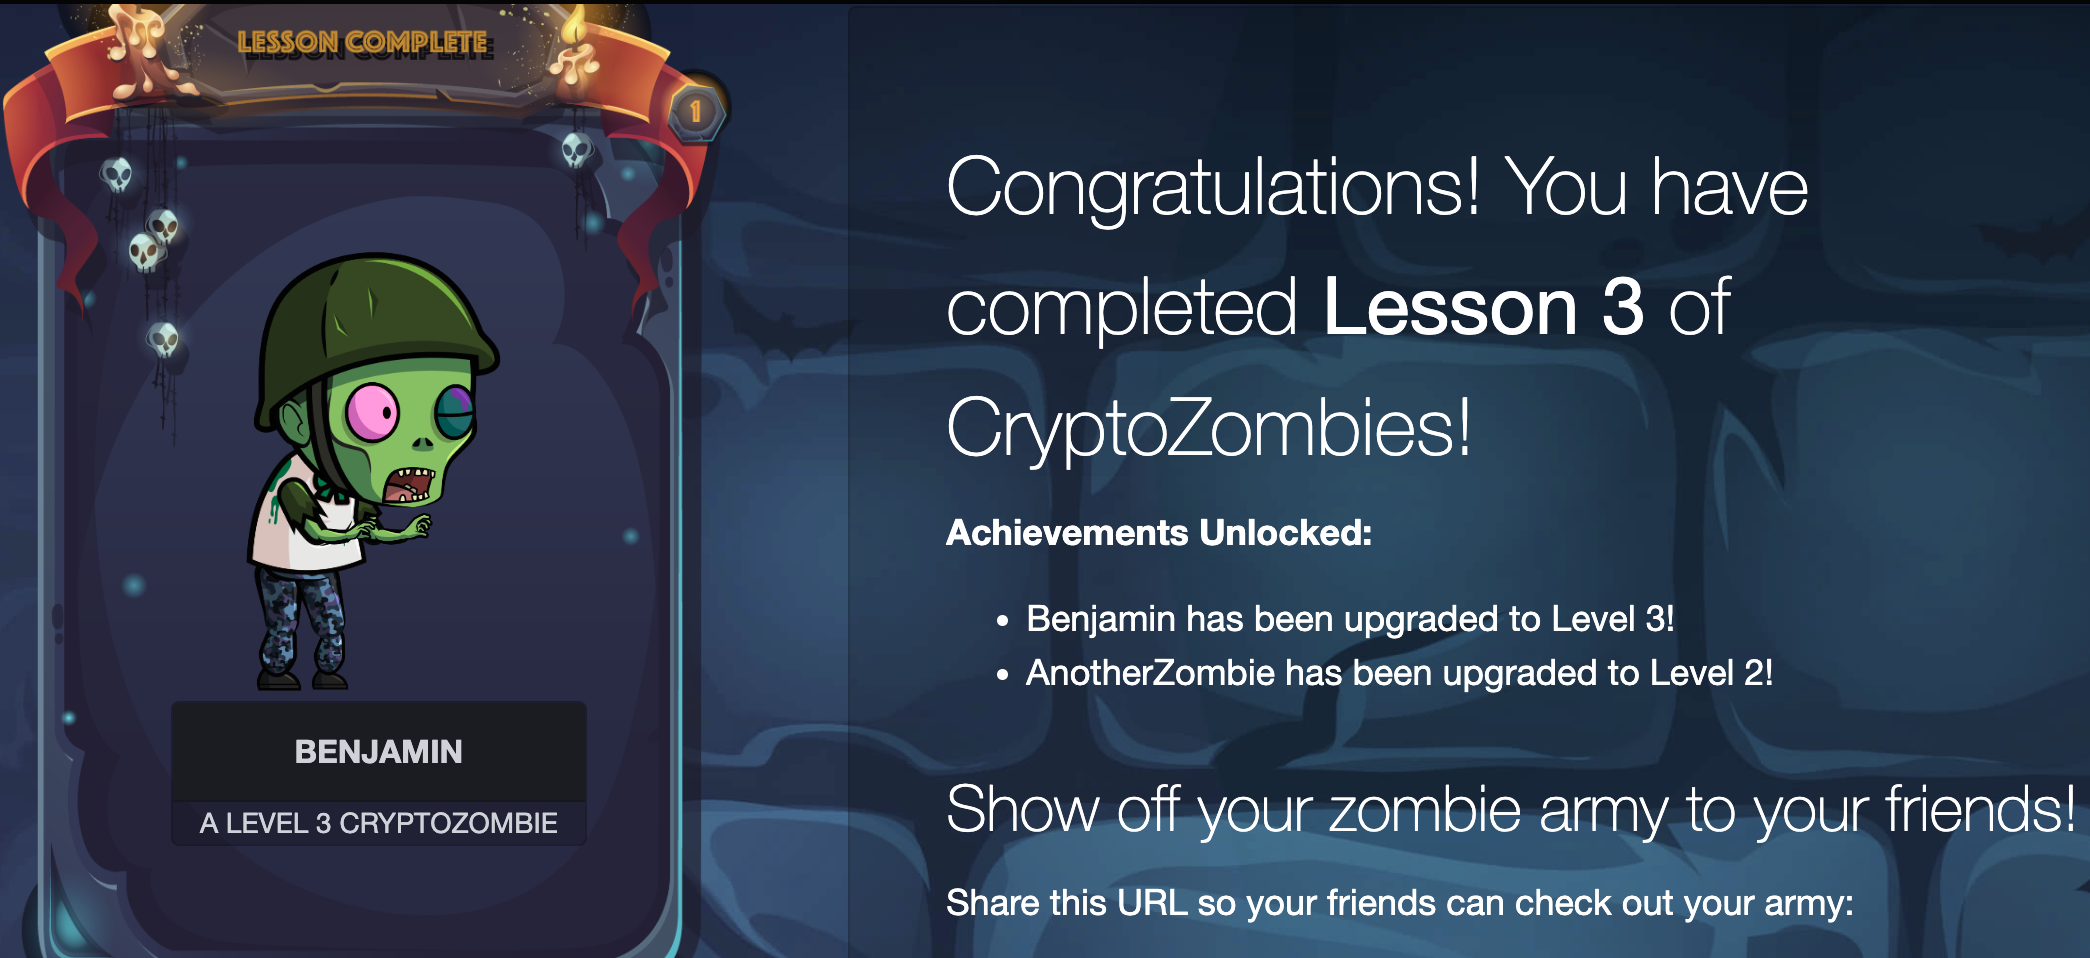
\includegraphics[width=\textwidth]{images/lesson3.png}

	\section*{Lesson 4}
	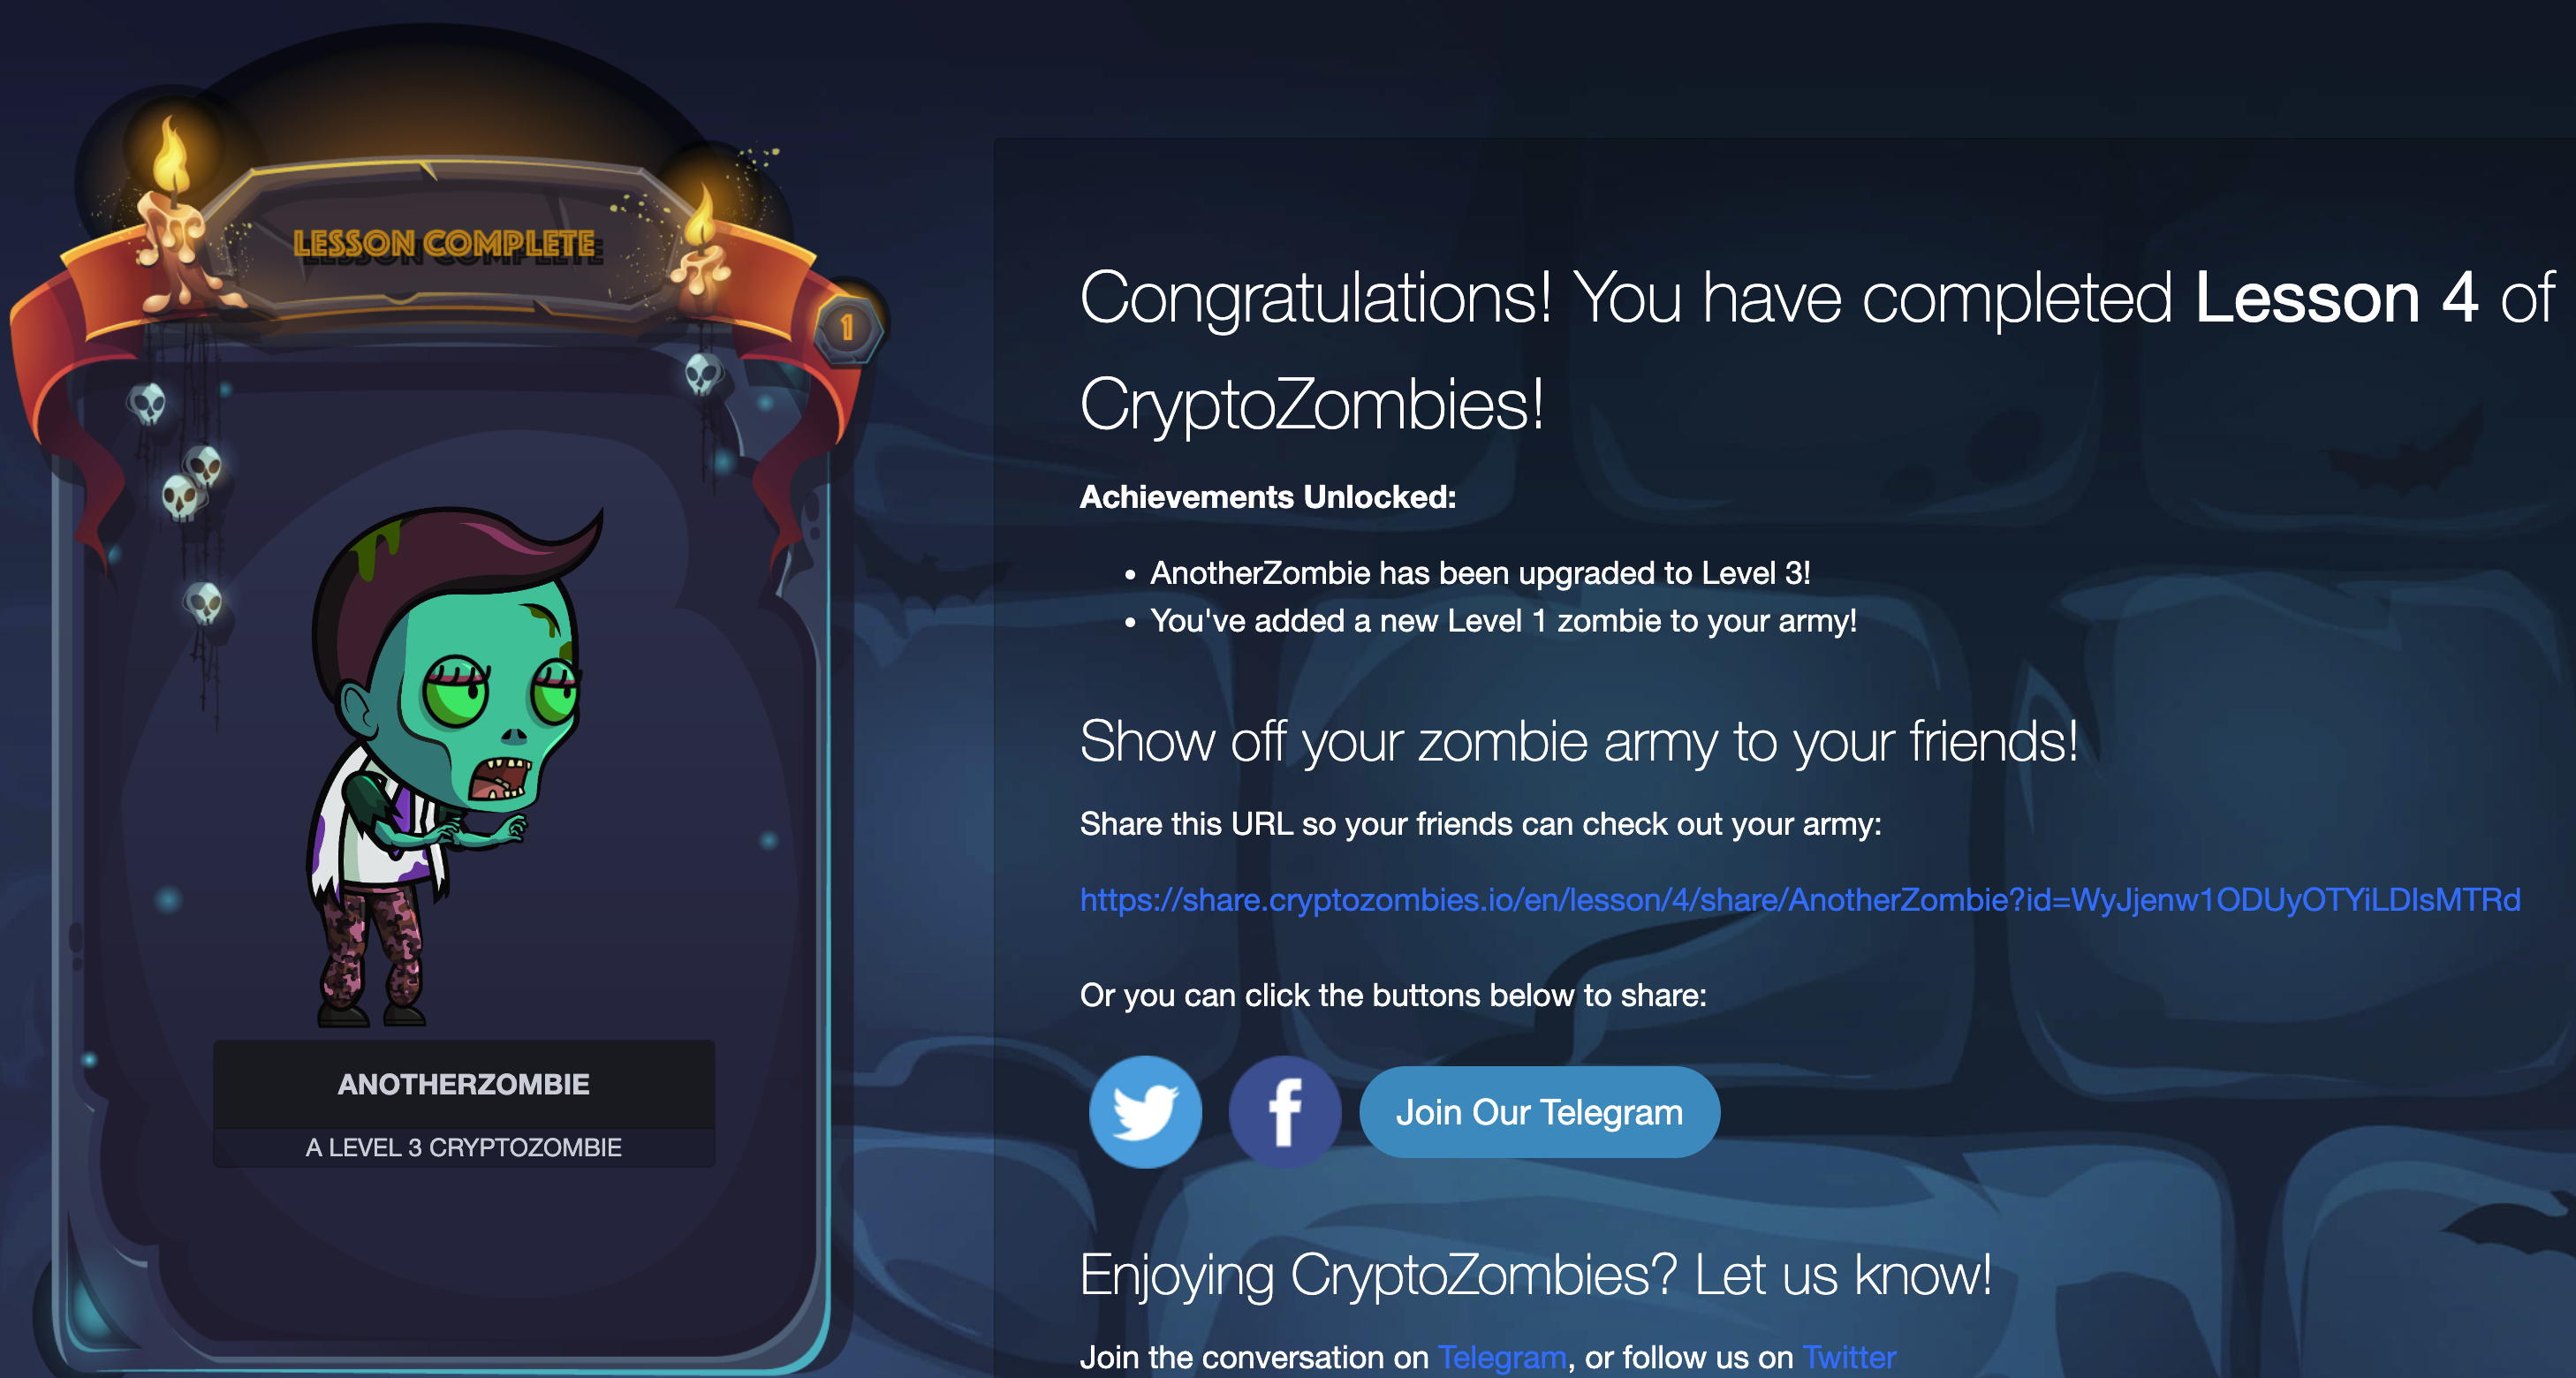
\includegraphics[width=\textwidth]{images/lesson4.png}

	\section*{Lesson 5}
	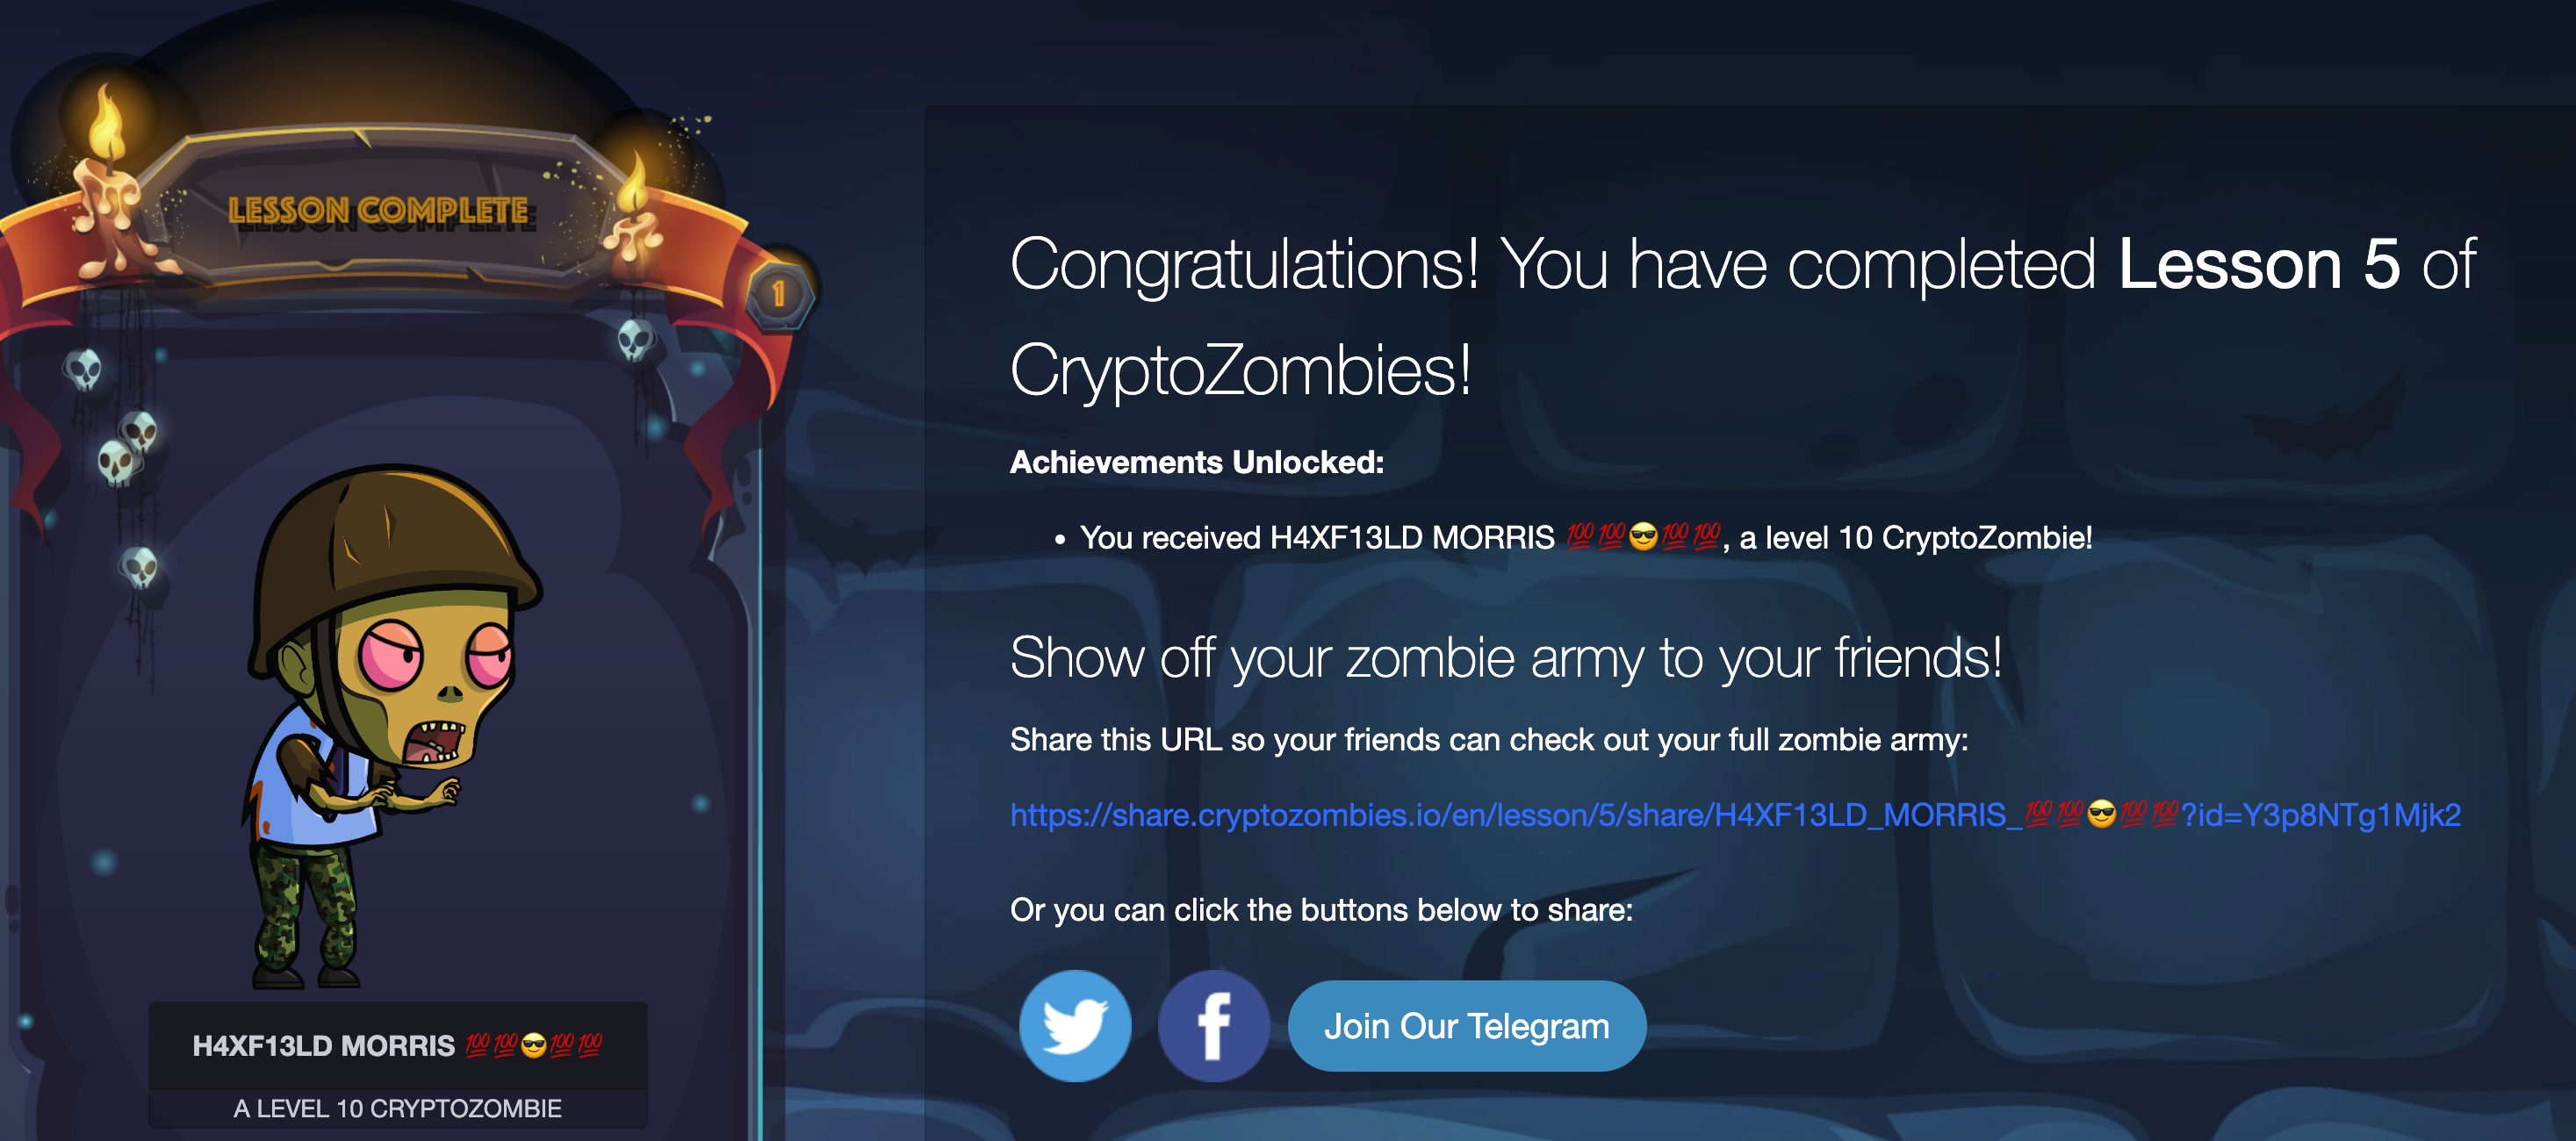
\includegraphics[width=\textwidth]{images/lesson5.png}

	\section*{Lesson 6}
	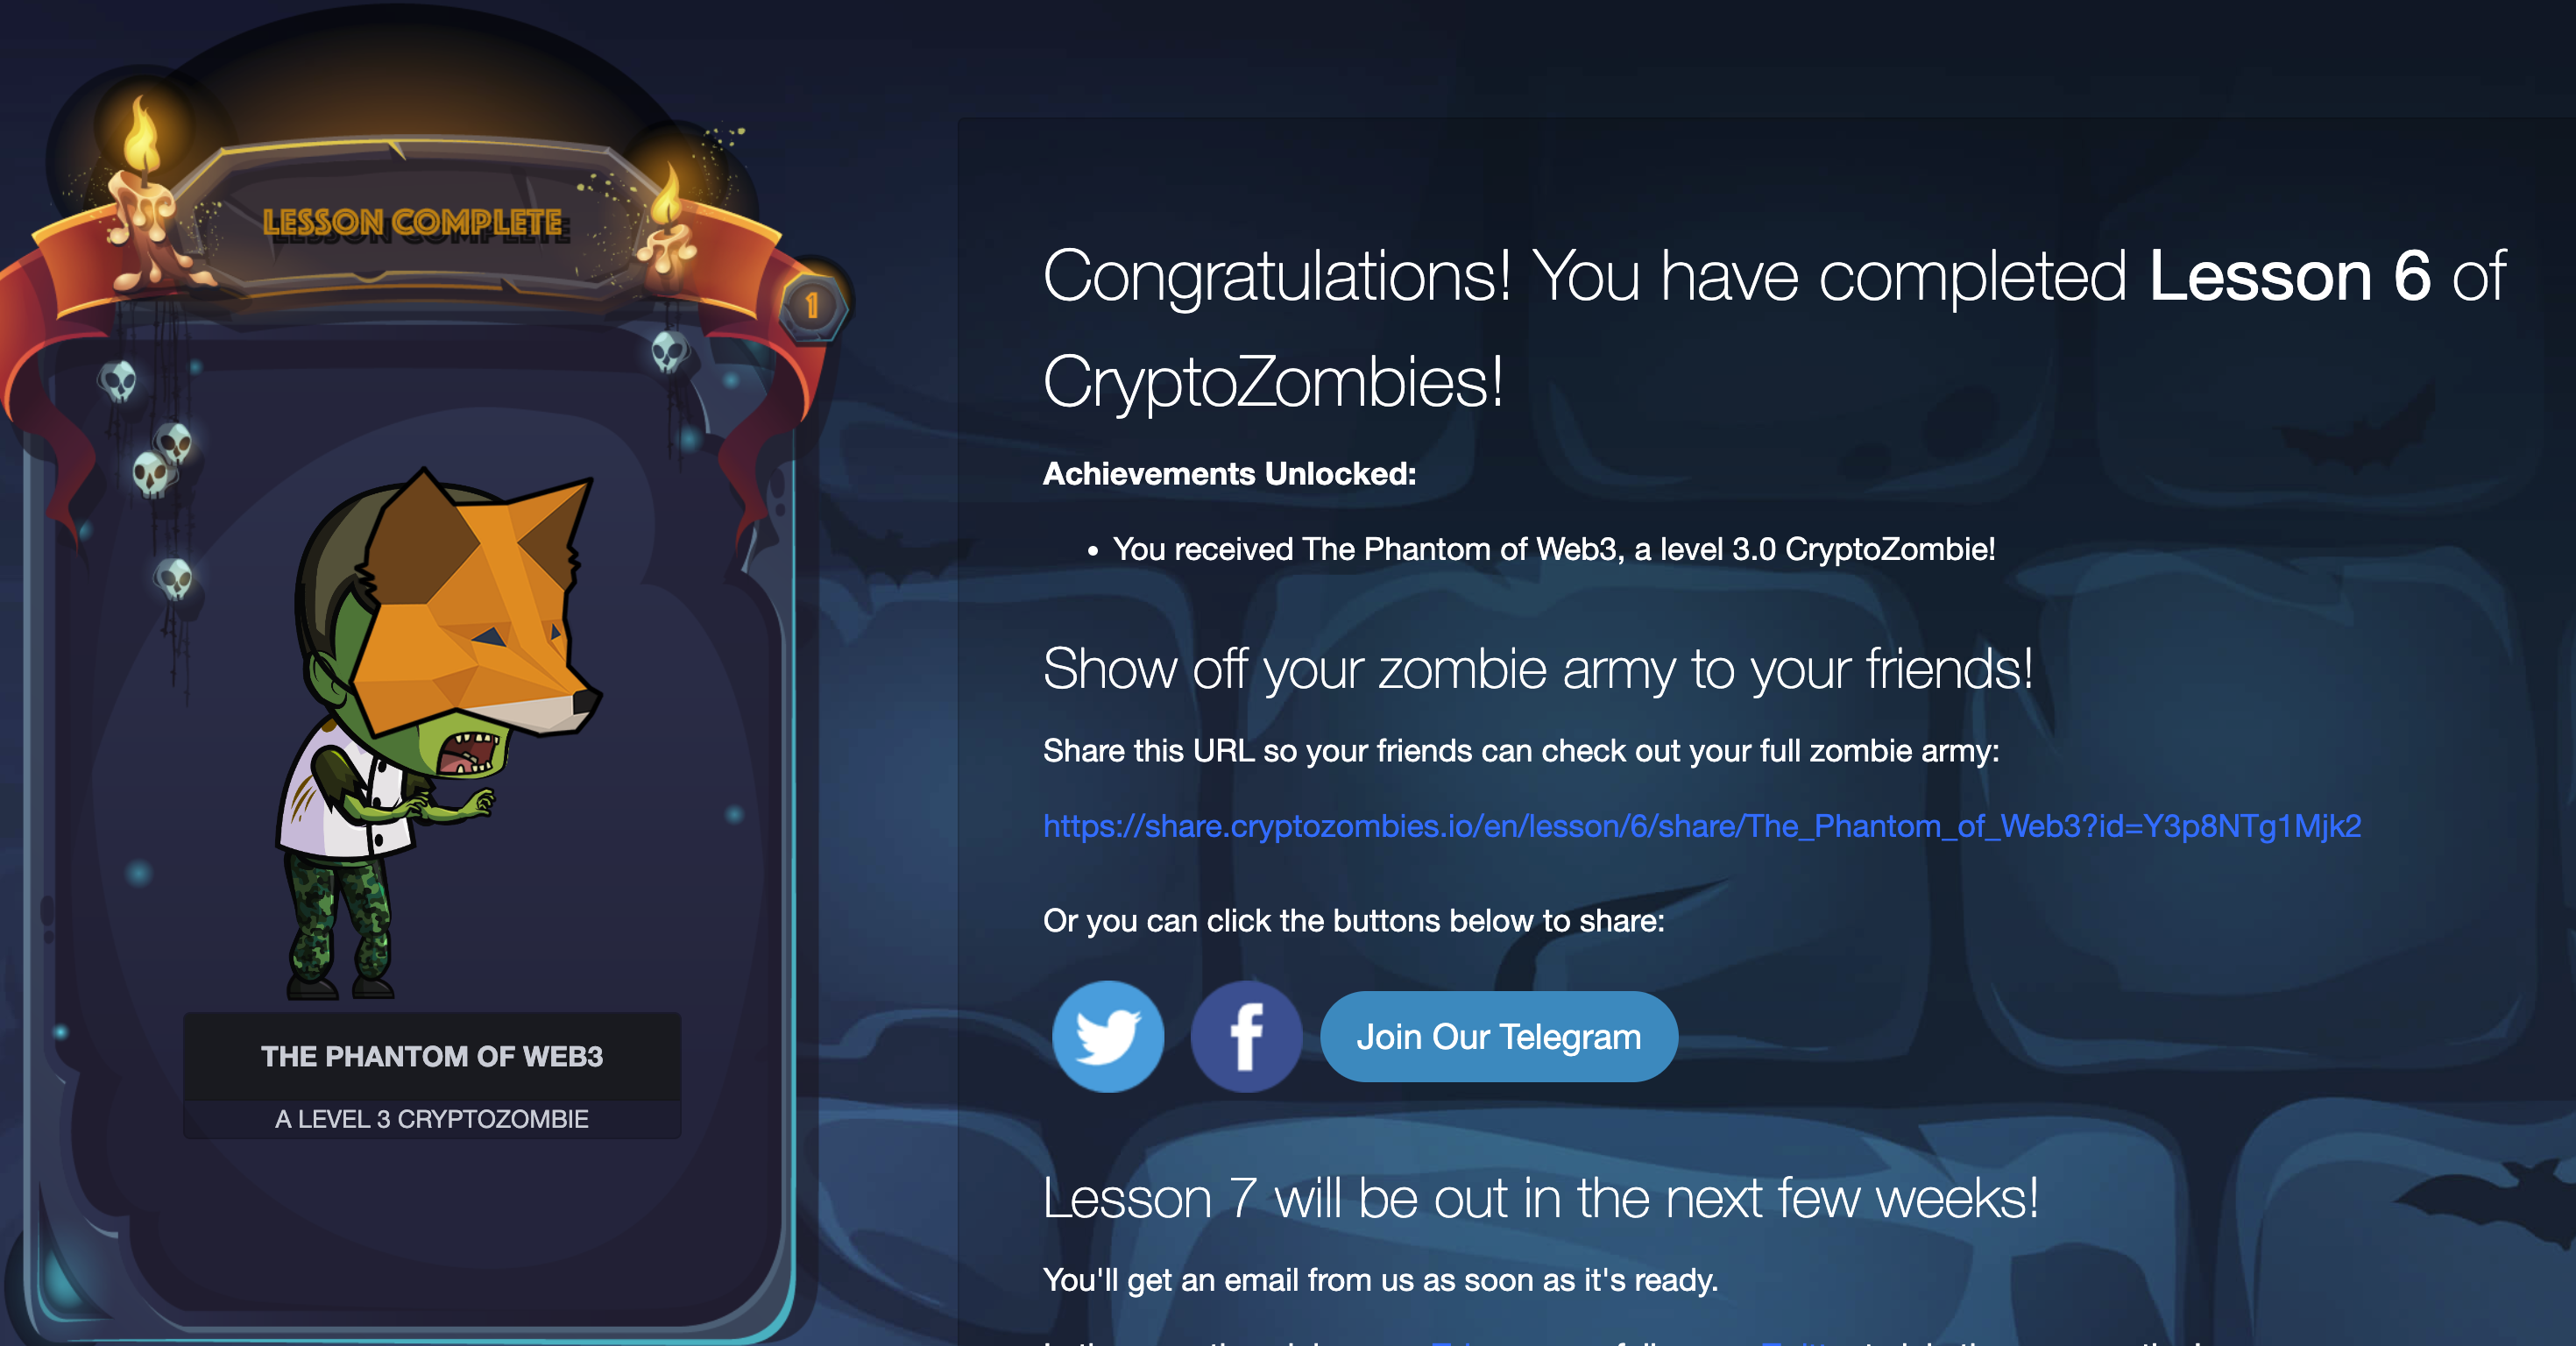
\includegraphics[width=\textwidth]{images/lesson6.png}

	\section*{All}
	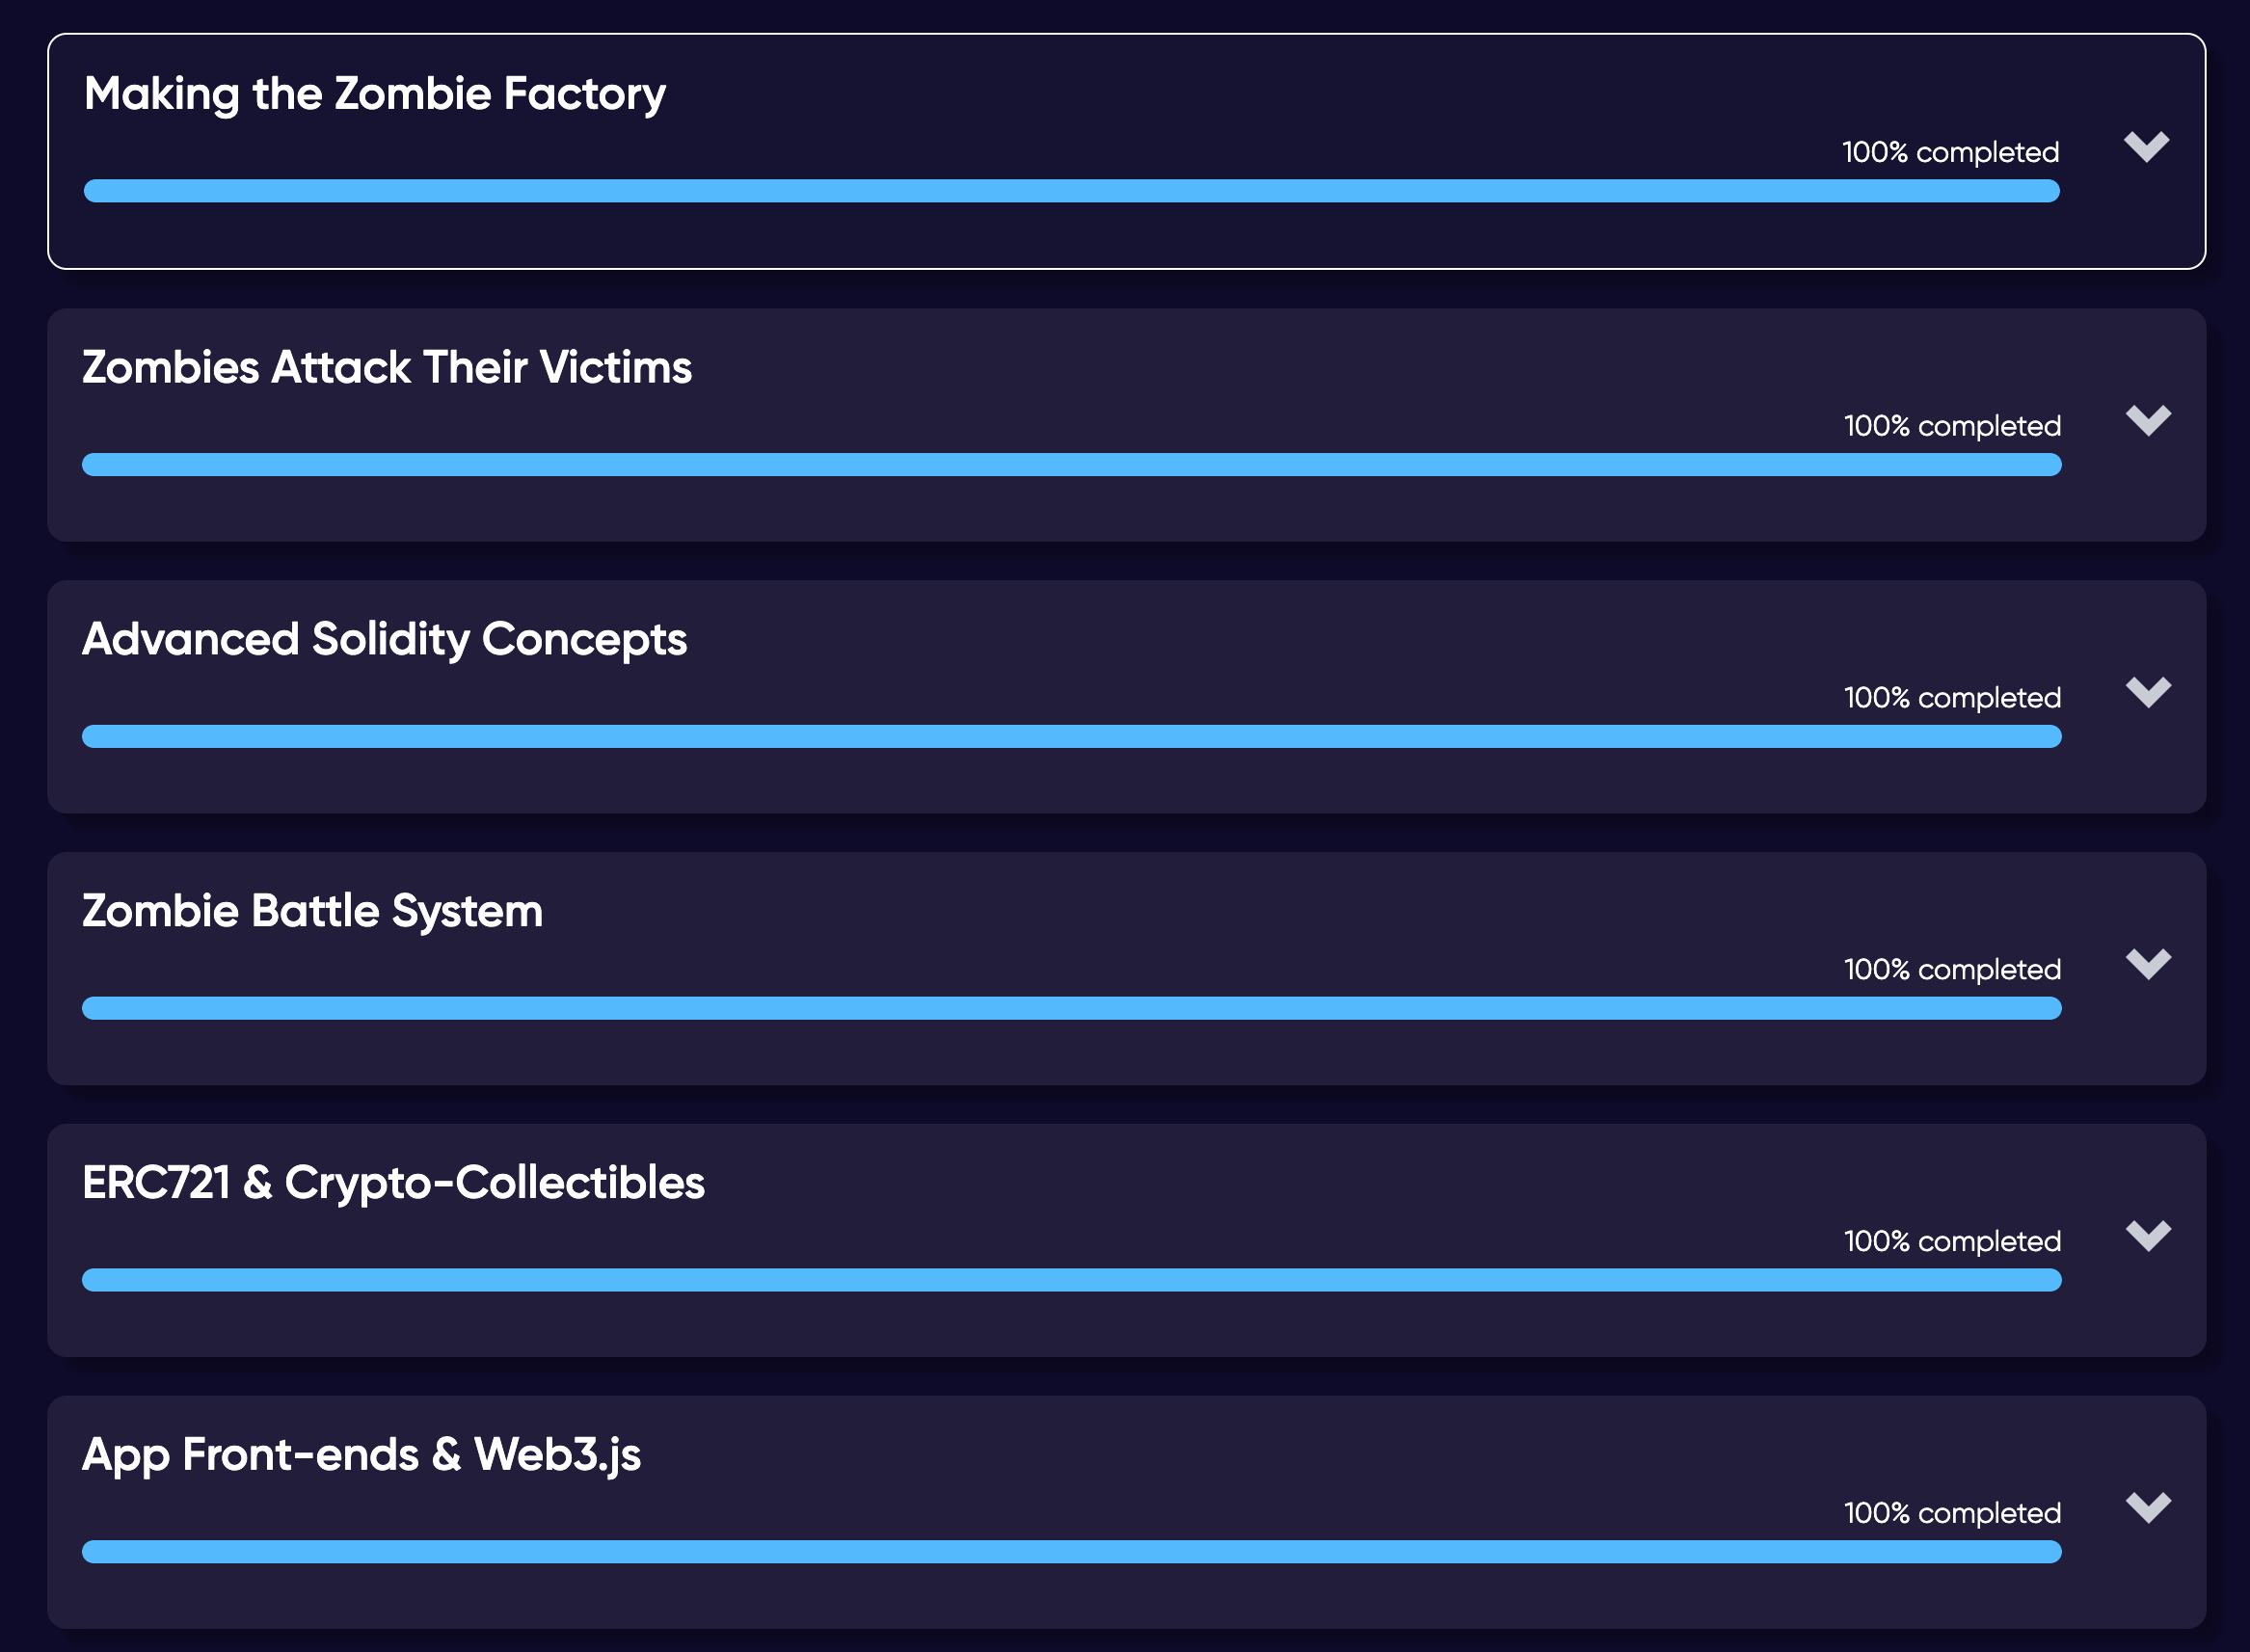
\includegraphics[width=\textwidth]{images/all.png}

\end{document}
